\chapter{Design}
In this section we present the design of our software application MusicDAO. MusicDAO is a mobile music streaming and discovery app, with peer-to-peer payment to artists in the form of donations and subscriptions. The MusicDAO is fully decentralized by design. This means there are no intermediaries, third parties or proprietary servers needed. All users of the app form a community to share audio tracks and transfer money. Any user can join this community, publish their musical works and receive money from its listeners. With the goal of distributing power in the music industry, every peer in the network will have the same rights and access to the same functions. All participants cooperate in the network, which makes it self-scaling by design.

The overall design of the system can be seen in fig. \ref{fig:architecture}. This describes the interaction between the different components, libraries and frameworks. The following sections explain the designed features, components and design choices.

\begin{figure}
    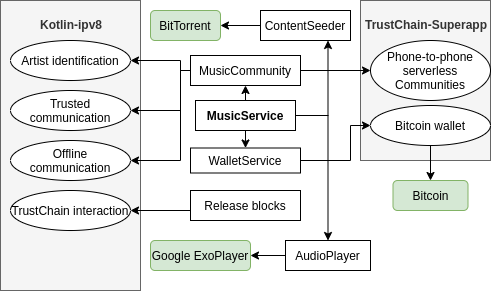
\includegraphics[width=0.6\textwidth]{design/architecture-v1.png}
    \caption{Architecture overview, with in green the external libraries. MusicService is the central component in our system}
    \label{fig:architecture}
\end{figure}

\section{Serverless architecture}
The network we are designing cannot use central servers or servers from third parties. This network should allow listeners and artists to exchange music and money, without the help from external services. We choose to build a phone-to-phone serverless network, for the following reasons. Firstly, Mobile phones have the largest share of any type of device using music streaming services. Secondly, if the software that we design and implement runs well on a network consisting of only mobile devices, we can conclude that it will run well on better hardware (such as PCs) as well. 

We choose to use the Android framework for decentralized apps as proposed by~\cite{mattskala2020}. This gives us a toolbox for building phone-to-phone serverless apps and make use of its distributed ledger technology to build a public database. It also gives us a public-key infrastructure to identify and authenticate artists. 

\section{Open protocol and artist freedom}
The design of our system contains both an open protocol and an application for the end-user. This is inspired by the ideas from \cite{masnick2019protocols}, who describes that the Internet should go back to open protocols instead of platforms, and that there should be a clear distinction between applications and protocols, so that users have the choice between different applications. Then, every application can have its own strategy of content moderation.  This should result in more competition to ``[...] provide better services that minimize the impact of those
with malicious intent, without cutting off their ability to speak entirely''~\citep{masnick2019protocols}.

In our context, we envision different applications using the same streaming, discovery and payment protocol, but with each application having strategies for content filtering and user interfaces. This way, music can not be censored in a centralized manner. Moderation of content happens on the side of the application, so that the user is in control of the settings of moderation and we do not lose freedom of speech or data resiliency.

\section{End-to-end music delivery model}
\label{sec:release-model}
In contrary to the current music publishing situation, dominated by IT gatekeeping and oligarchs as visualized in fig. \ref{fig:current-music-publishing-situation}, we present the desired situation in fig. \ref{fig:desired-music-publishing-situation}. This shows the liberation for artists in publishing their content, and the reduction of single-point-of-failure risks. In this system, artists are free in what they upload. In addition, their content can not be taken down by any authority unless there are no participants in the network. The discovery of content is done using open source, transparent systems and listening data is saved and processed locally.

To achieve this situation, a main component of our system is the storage of metadata and audio files for playlists. We design an abstract model for the structure of this metadata, so that the artist is free in the way to release music content. The artist may publish tracks as part of a single, an EP, an album or any other structured list of tracks, as a Release object.

\begin{figure}
    \centering
    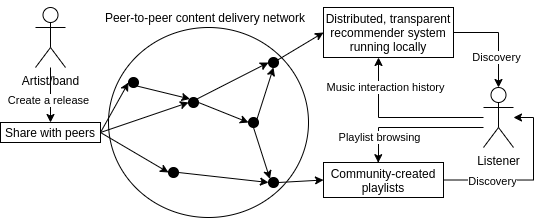
\includegraphics[width=0.8\linewidth]{design/desired-music-publishing-situation.png}
    \caption{Desired music publishing flow using a distributed network}
    \label{fig:desired-music-publishing-situation}
\end{figure}

A Release object contains a list of tracks that are published by a clearly identifiable artist or group of artists. It is modeled as shown in fig. \ref{fig:release-model}. Release objects are shared between peers in the network. By discovering many of those objects, a user can see and browse through them to select a track to play. A Release object merely contains metadata of the tracks. We design the network to have a separate channel for downloading the track files. This is to enable fast discovery and
searching of Releases, as Release objects have a small byte size. 
\begin{figure}
    \minipage{0.2\textwidth}
        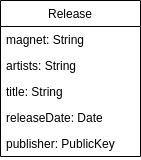
\includegraphics[width=\linewidth]{design/release-model.png}
        \caption{Release blocks structure as seen on TrustChain}
        \label{fig:release-model}
    \endminipage\hfill
    \minipage{0.3\textwidth}
        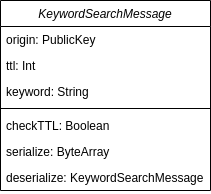
\includegraphics[width=\linewidth]{design/KeywordSearchMessage-model.png}
        \caption{KeywordSearchMessage object sent over IPv8 in MusicCommunity}
        \label{fig:keyword-search-message-model}
    \endminipage\hfill
    \minipage{0.5\textwidth}
    \endminipage
\end{figure}

\section{Permissionless infrastructure and identities}
\label{sec:pki-design}
The MusicDAO allows any person to participate, and start publishing or listening to music. It requires a permissionless infrastructure, in which artists can be identified. As we design a system that is fully decentralized, we cannot use a central database to record user identities. Therefore every user generates a unique identity to be used in the network, and must be able to give proof of this identity. We use a public key infrastructure (PKI) which achieve these goals. Every user stores their private and public key on their device, and only share their public key. The keypair has a mathematical property that allows verification of messages that are signed with a private key. By comparing the public key of a peer with their signed message, anyone can verify the authenticity of the message.

In the context of MusicDAO we use this PKI to proof ownership of Release objects. All Release objects are signed using the owner's private key and the signature is added to the object. Any user receiving this object can verify its authenticity.

We choose to use the public key infrastructure as implemented in the TrustChain-Superapp~\citep{mattskala2020}. This gives us a unique identity per Android phone, by abstracting the network identities such as (changing) IP addresses and Bluetooth addresses. 

\section{Distributed storage}
\label{sec:distributed-storage}
Central to our system is sharing downloading and storage of audio files and Release objects (see \ref{sec:release-model}). To design a system which has no middlemen or regulators for publishing Releases, and has no central control, a distributed storage system is required. This storage system should have the following properties: immutability (data cannot be tampered with), resiliency (data should be available as long as users want it) and rigorous duplication (all objects should be saved on multiple machines). Distributed ledger technology (DLT) allows for these properties, so we design our system with a DLT as a major component.

One implementation of this technology is TrustChain~\citep{otte2017trustchain} which allows for recording transactions between peers in a linearly scaling public ledger. Every peer has its own immutable and public blockchain which shows its history of transactions with others. This way we can establish trust in a certain party. In our context, we can use this mechanism to estimate trust in artists by inspecting their public history of uploads. We choose TrustChain because of its scalability, its trust mechanism, and because it has a native implementation for Android, as described in \ref{sec:sote-trustchain}. In addition, this implementation allows for offline communication, so users can download and explore new content using Bluetooth or LAN.

\section{Distributed music sharing}
To be able to have low latency for discovering and playing music tracks, while using no central nor high-throughput servers, the network demands participants to upload content continuously. We design the app to, by default, use the network capabilities of the mobile device to upload content as much as possible. This is constrained by networking hardware, data subscription plans and other software running on the phone.

The peer-to-peer file sharing protocol BitTorrent is suitable to share audio files in MusicDAO. We make BitTorrent a design choice as it does not require synchronizing with a global data store, in contrary to IPFS. This means we can build a metadata store independently from BitTorrent (for example, using TrustChain as explained in \ref{sec:distributed-storage}). BitTorrent also has stable implementations for Android.

\section{Distributed search algorithm}
For searching content we use introduce our simple distributed algorithm. Pseudocode of this algorithm is shown in algorithm 1. It asks peers around for content tagged with some keyword. When a peer finds a match on their local database, it sends this Release object to the original asking peer. Otherwise it forwards the query to their neighbours, after reducing the time-to-live property by 1. The messages stop being forwarded once their time-to-live property hits below 1. The structure of search messages are shown in fig. \ref{fig:keyword-search-message-model}.

\section{Transparent money flow}
Figures \ref{fig:current-money-flow} and \ref{fig:desired-money-flow} visualize, in a simplified fashion, the difference of how money flows in the current situation and in MusicDAO. It shows that, when intermediaries are cut from the flow, artists will have a higher income for the same fees from the listener. Streaming services and record holders introduce many overhead costs. Our system allows artists to publish their songs without the need to contact a label. The biggest difference in income will be seen for independent artists, as streaming services gives particularly low payouts for unsigned artists.

As we are designing a system with no intermediaries, it should be possible to give money directly to artists. Cryptocurrency allows for peer-to-peer payments which achieve this goal, so we use this in the MusicDAO. Cryptocurrency payments will be used for two different functionalities: a user can send a donation to an artist, or a user can pay artists using a monthly subscription system. This subscription system pays artists that the user listened to, using the Artist Income Division Algorithm (see \ref{sec:aida-design}). 

In the desired money flow, we have a  Fig. \ref{fig:desired-money-flow} shows another component: an automated and transparent payment division system. In practice, this should be an algorithm running locally on the machine of the user which calculates how much money should go to each of the shareholders of a particular song. Currently, record holders have this task, but there exists no transparent system for this, so they can give low payouts to its artists. We design the transparent payment system to be an immutable record on a distributed ledger, on which a specification of the exact shares per artists are written down. This can be implemented using TrustChain blocks~\citep{otte2017trustchain}.

We choose to use Bitcoin as a cryptocurrency as it has shown to be a secure and popular payment system, and it does not rely on any third parties to run. It also allows for making a experimentation environment without any high-throughput external servers. 

\begin{figure}
    \minipage{0.6\textwidth}
        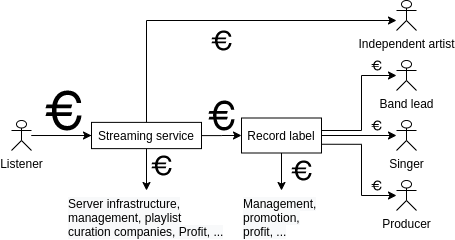
\includegraphics[width=\linewidth]{design/current-money-flow.png}
        \caption{Money flow: current situation (simplified)}
        \label{fig:current-money-flow}
    \endminipage\hfill
    \minipage{0.4\textwidth}
        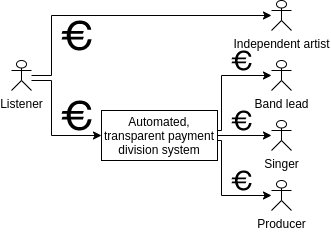
\includegraphics[width=\linewidth]{design/desired-money-flow.png}
        \caption{Money flow: desired situation}
        \label{fig:desired-money-flow}
    \endminipage
\end{figure}
\subsection{Wallet}
Cryptocurrency implementations allow for private/public key-pairs which can be interpreted as a kind of wallet; the funds can only be unlocked by a holder of the private key. In the case of MusicDAO we design the app to include a wallet for every user. To receive money, every artist should share their public key to all of their listeners. To achieve this, the public key of their cryptocurrency wallet is included as a property of the Release objects (see \ref{sec:release-model}). As there are no institutions or banks involved in storing money, users will be required to keep their private key safe.

\subsection{Artist Income Division Algorithm}
\label{sec:aida-design}
To provide a stable income for artists, in the form of reoccurring payments, we design the Artist Income Division Algorithm. This algorithm calculates how periodic subscription money is split into payments to artists. The user can enable a periodic payment. This money is then divided over the artists the user listens to, in proportion to the amount of interaction with each artist. Interaction can be measured in e.g. time listened, plays or feedback in the form of likes. The details of this division is explained in the implementation section of AIDA (see X).

\begin{algorithm}
\caption{Distributed algorithm for remote search}
\begin{algorithmic}
\Function{DistributedSearch}{$query, ttl, maxPeers, minResults$}\Comment{Device initiates the search}
    \State $results\gets localSearch(query)$\Comment{Filter local database}
    \If {$|results|\leq minResults$}
        \State $origin \gets myAddress()$\Comment{Address of the device initiating the search}
        \For{$i\gets 1, maxPeers$}
            \State $peer \gets peers[i]$\Comment{Select a random neighbor}
            \State $sendQuery(origin, peer, query, ttl)$
        \EndFor
    \Else
        \State \textbf{return} $results$
    \EndIf
\EndFunction
\Function{OnQuery}{$origin, peer, query, ttl$}\Comment{This is called when a query is received}
    \If $ttl\leq 0$
        \State \textbf{return}
    \EndIf
    \State $ttl \gets ttl-1$
    \State $results\gets localSearch(query)$
    \If {$|results|\le 1$}
      \For{$i\gets 1, maxPeers$}
            \State $peer \gets peers[i]$
            \State $sendQuery(origin, peer, query, ttl)$
        \EndFor
    \Else
        \State $sendResults(origin, results)$\Comment{Send the results back directly to the origin}
    \EndIf
\EndFunction
\end{algorithmic}
\end{algorithm}

% \section{Splitting the application and data layers} Mention the protocol vs platform model by Masnick
